%****************************************************************************
%** Copyright 2002 by Lukas Ruf, ruf@topsy.net
%** Information is provided under the terms of the
%** GNU Free Documentation License http://www.gnu.org/copyleft/fdl.html
%** Fairness: Cite the source of information, visit http://www.topsy.net
%****************************************************************************
%****************************************************************************
%** Last Modification: 2005-07-11 1600
%** 2005-07-11	Bernhard Tellenbach
%**							This is an addapted version of the Introduction.tex file
%**							Added table example (footnotes,multicolumn)
%**							Examples for different text sizes
%**							Updated eps file inclusion example for use with graphicx pkt. 
%****************************************************************************

\chapter{\label{chapter2}Background}

\section{\label{chapter2:iSDX}iSDX}
The iSDX is a framework for deploying software defined networking at internet exchange points. \\
An internet exchange point is a physical location where multiple autonomous systems meet to exchange traffic and BGP routes. \\
Deploying the iSDX at an internet exchange point gives participants more control over routing decisions. This is done by giving participants the opportunity to define policies. These policies allow participants to influence traffic coming from and going in the internet exchange point without obscure BGP message manipulation. The iSDX uses an SDN switch connected to the iSDX and all the participants to implement the policies as flowrules.
\subsection{\label{chapter2:iSDX:policies}policies}
Policies match on a field of the packet header and then forward the packet to a participant.
\paragraph{\label{chapter2:iSDX:policies:outbound policies}outbound policies:}
Outbound policies let participants direct packets going from themselves to the iSDX. They allow the participants to choose the participant the packet gets sent to.
\paragraph{\label{chapter2:iSDX:policies:inbound policies}inbound policies:}
Inbound policies allow participants to direct packets coming from the iSDX. In effect they allow the participant to choose to which of his own routers packets from the iSDX get sent to. 

\begin{figure}[h]
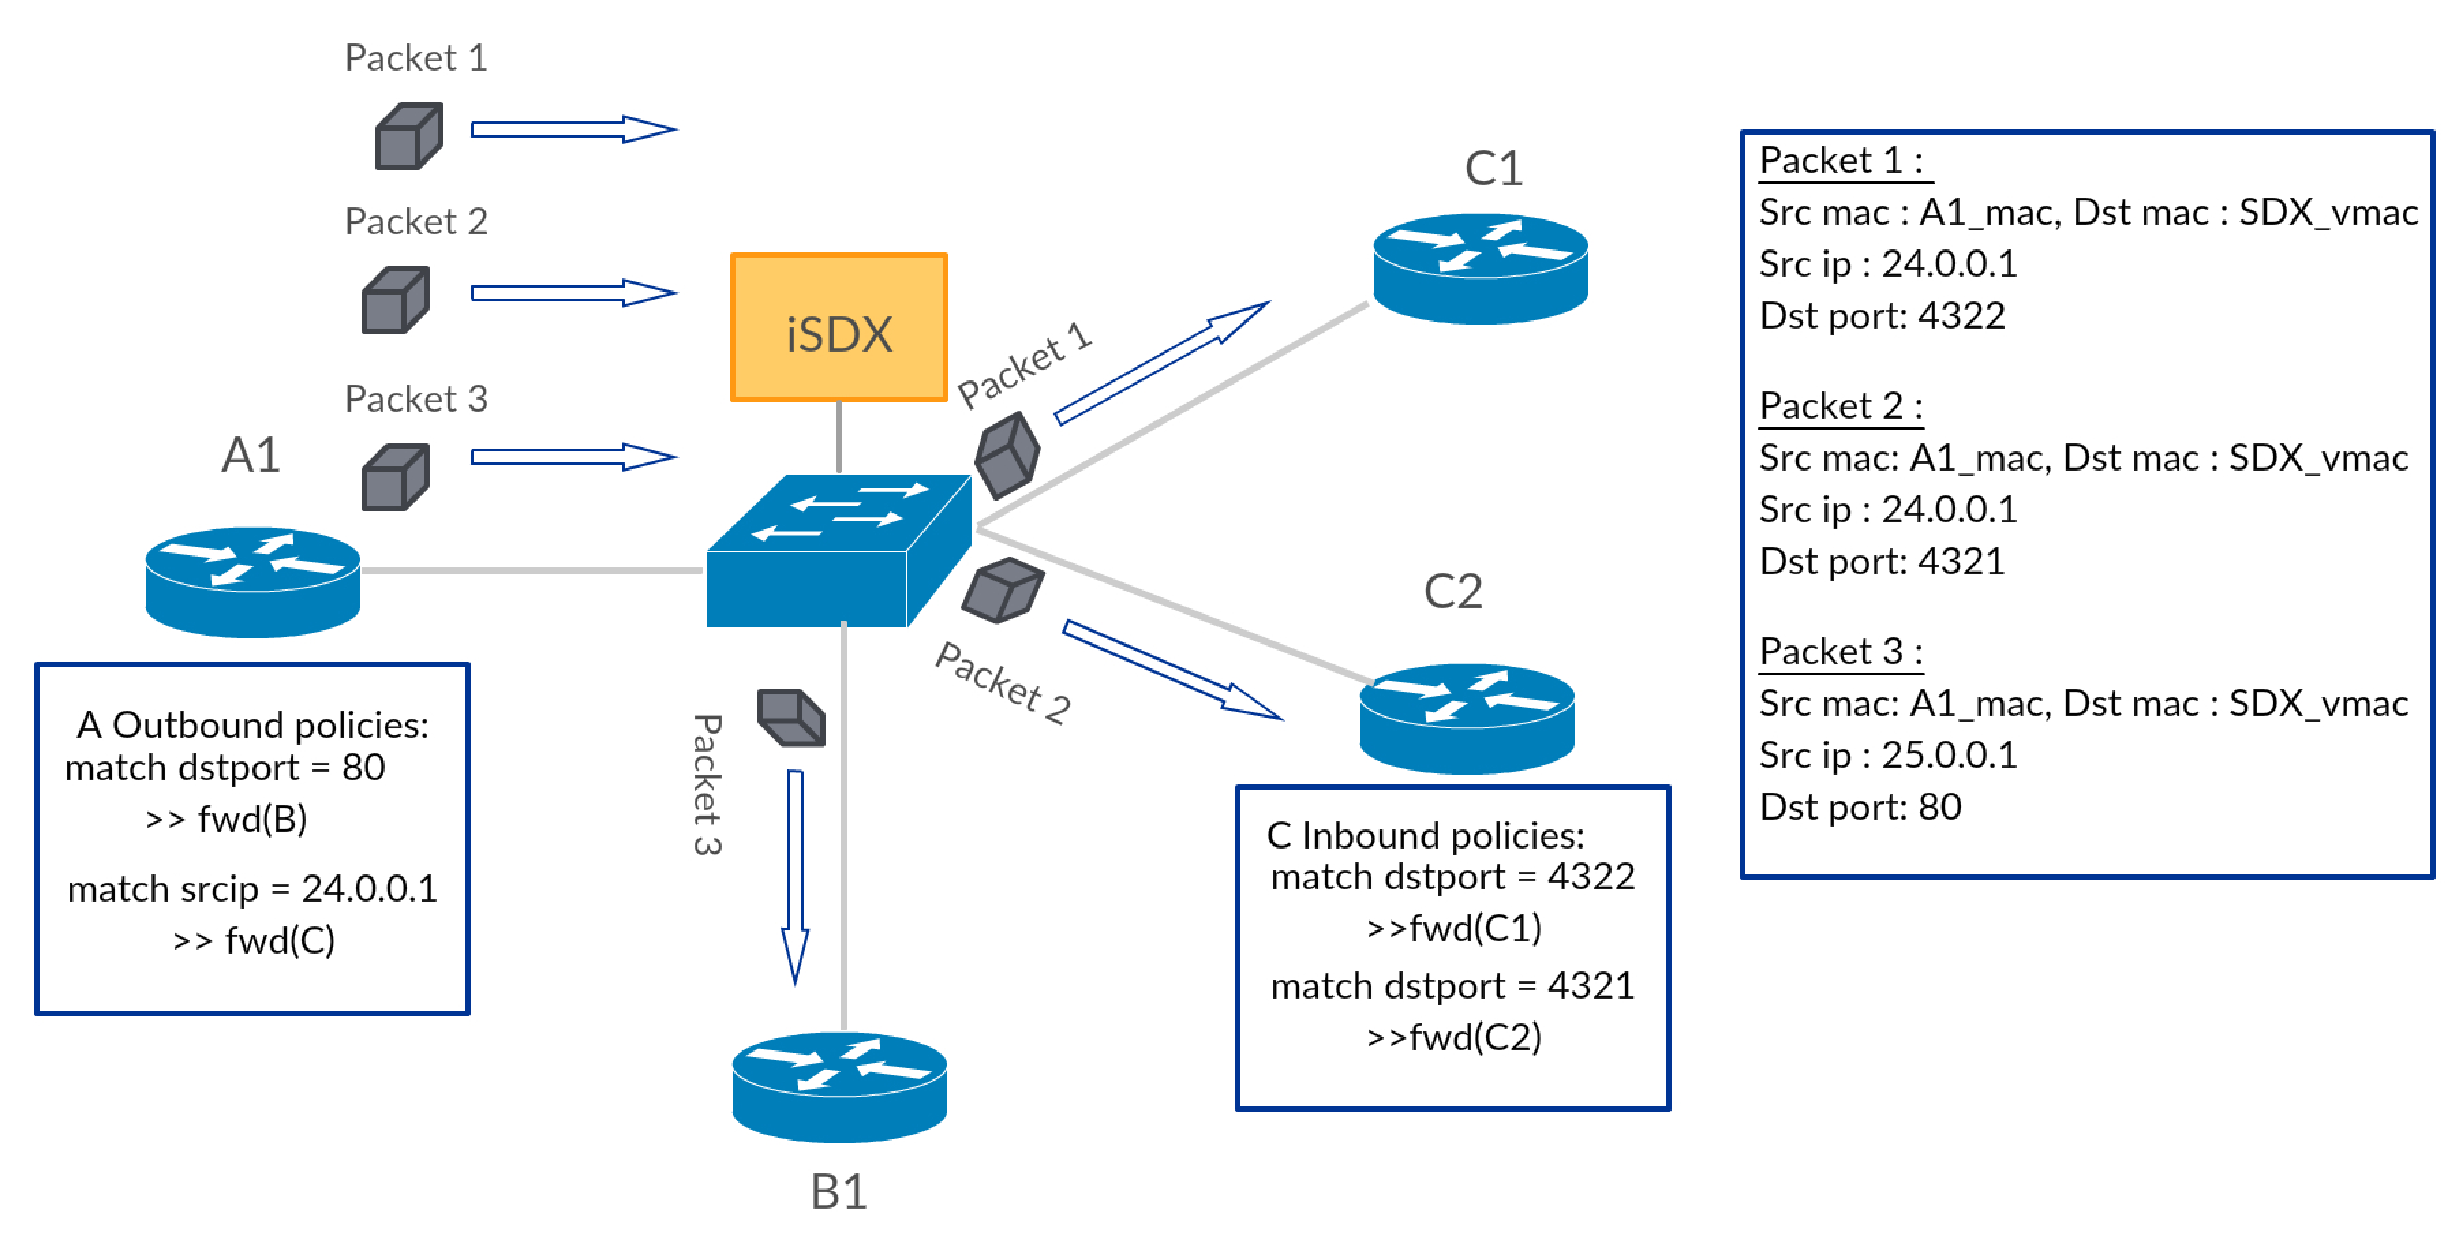
\includegraphics[scale = 0.32]{C:/Users/Philipp/SemesterProject/report/Figures/bckgrnd_sdx_policies.pdf}
\caption{Example of outbound and inbound policies with an iSDX connected to three \\ participants}
\end{figure}


\subsection{\label{chapter2:iSDX:virtual next-hop, virtual mac address}virtual next-hop, virtual mac address}
In order to not violate BGP advertisements (send packets to participants that did not advertise the prefix of the packet) the iSDX uses the destination mac address as a data plane tag. \\ 
In the destination mac address the iSDX encodes the participants advertising the prefix of the packet and the BGP best next hop participant for this prefix. This mac address corresponds to a virtual next hop, which is assigned to every prefix. \\ The iSDX sends BGP updates to the participants, with the next-hop of the update set to the virtual next-hop of the prefix. The virtual mac address is communicated to the participants via ARP.
\paragraph{\label{chapter2:iSDX:virtual next-hop :inbound policies}iSDX vmac:}

\begin{tabular}{|r|l|}
  \hline 
  participants advertising the prefix & BGP best next-hop participant \\
  \hline
\end{tabular}

\begin{figure}[h]
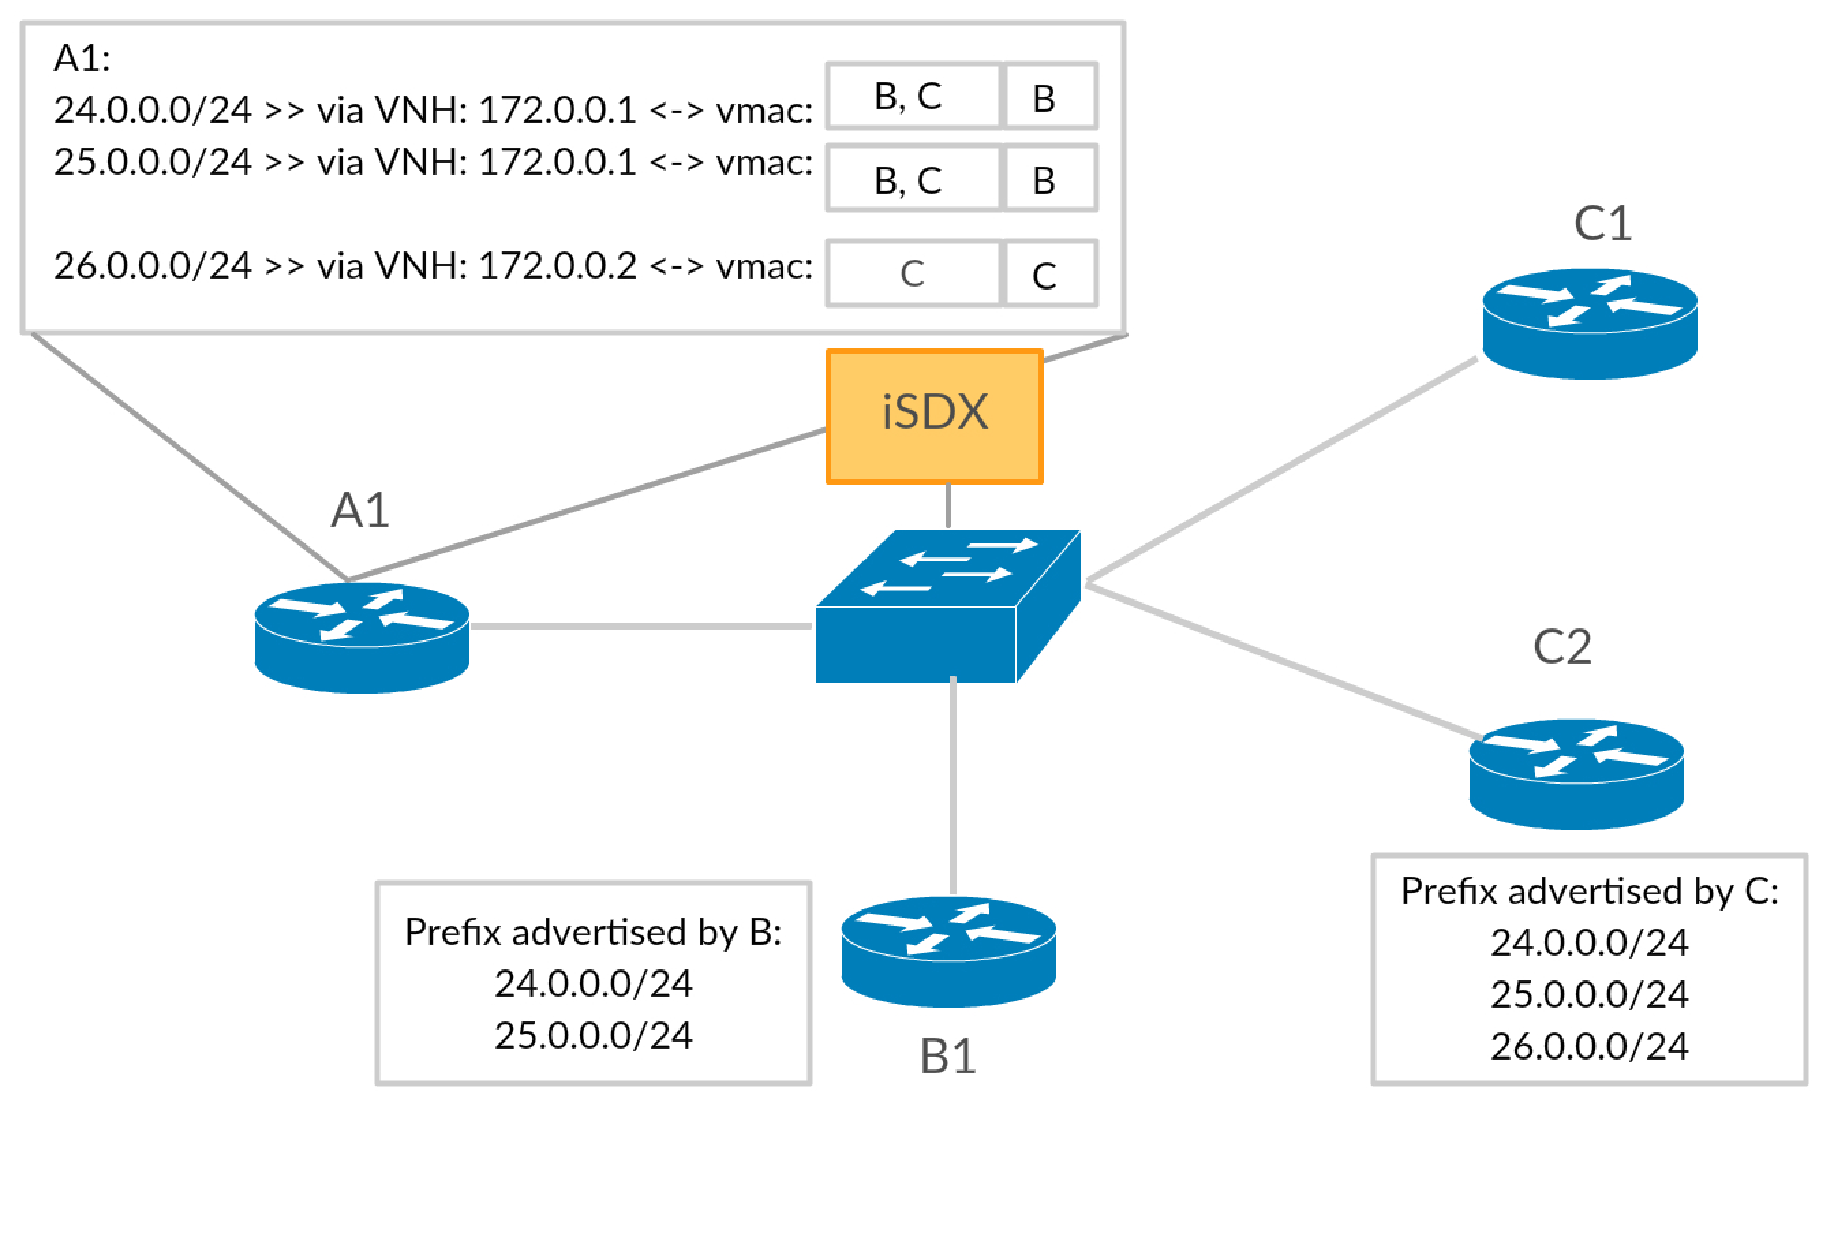
\includegraphics[scale = 0.36]{C:/Users/Philipp/SemesterProject/report/Figures/intro_sdx_vmac.pdf}
\caption{Example of the iSDX vmac with an iSDX connected to three participants}
\end{figure}

\subsection{\label{chapter2:iSX:iSDX architecture}iSDX architecture}
\begin{figure}[h]
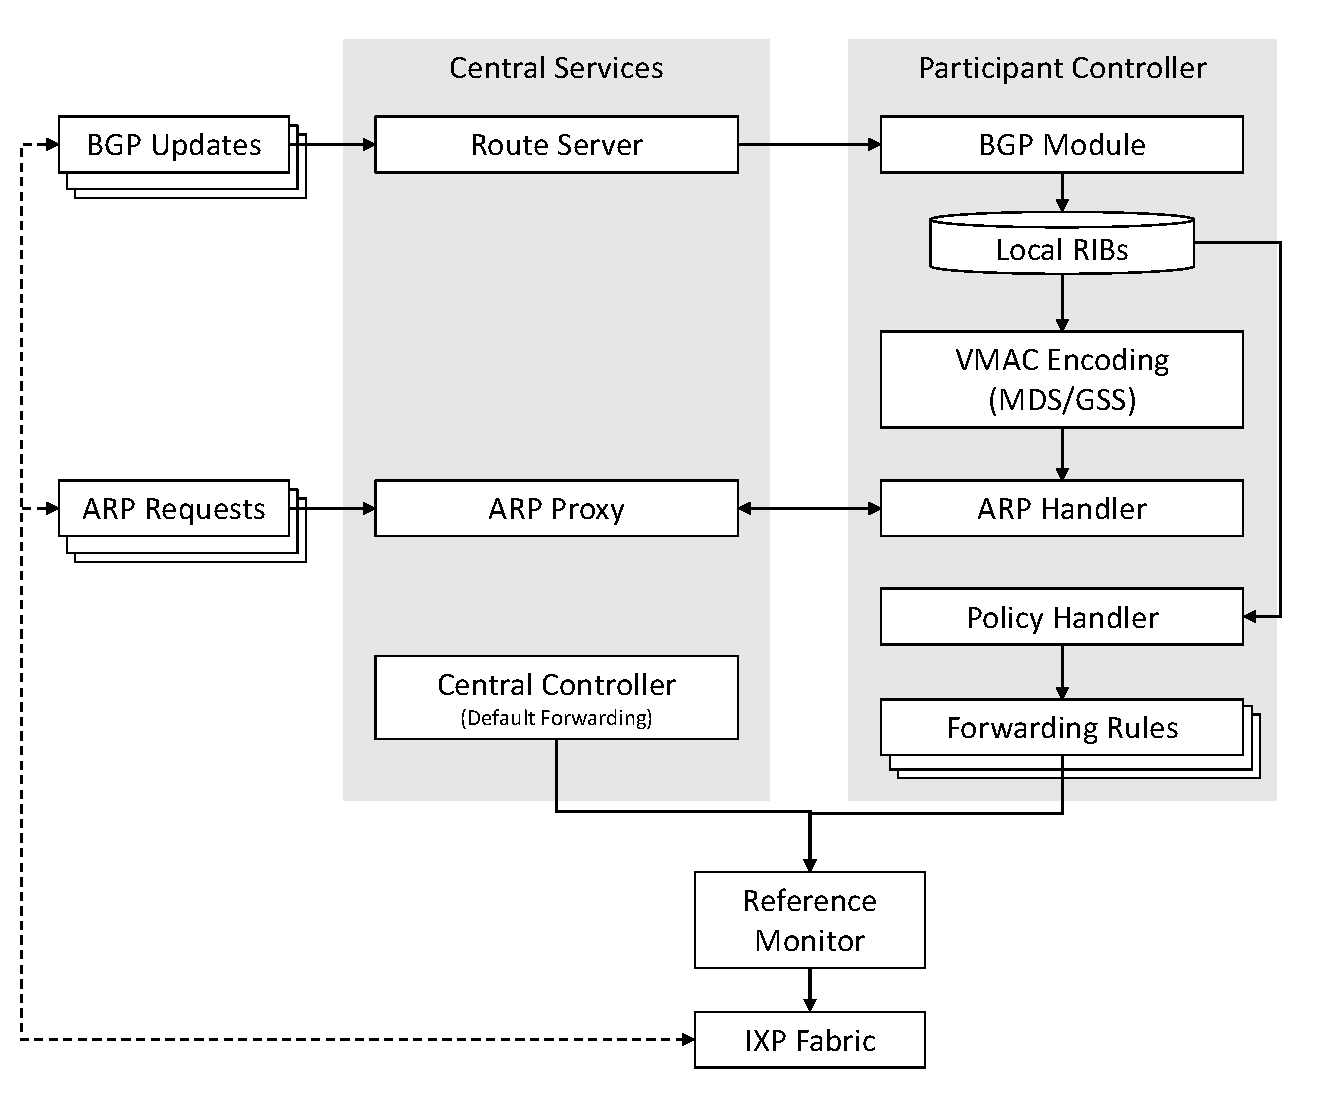
\includegraphics[scale = 0.4]{C:/Users/Philipp/SemesterProject/report/Figures/bckdgrnd_sdx_architecture_cropped.pdf}
\caption{iSDX architecture}
\end{figure}

The iSDX architecture has two main Parts. The Central Services and the Participant Controller. Every participant has its own participant controller. \\
Central Services forwards BGP updates and ARP queries to the corresponding participant controller. It also initializes all the static flow rules. \\
The participant controller receives BGP updates from the Route Server. It then actualizes it's RIB checks if the virtual mac address was changed by the received BGP update, if so sends a gratuitous ARP to the ARP proxy. The participant controller also manages each participant's inbound and outbound policies. 

\section{\label{chapter2:Swift}Swift}

Swift is a prediction and fast-reroute framework to improve the convergence time of a BGP speaking router upon remote failure. Swifts prediction relies on the fact that the cause of a burst of withdrawals can be determined before receiving all the withdrawals. \\ Swift uses a SDN switch connected to the swifted router, it's neighbors and to the Swift controller. 


\begin{figure}[h]
\center
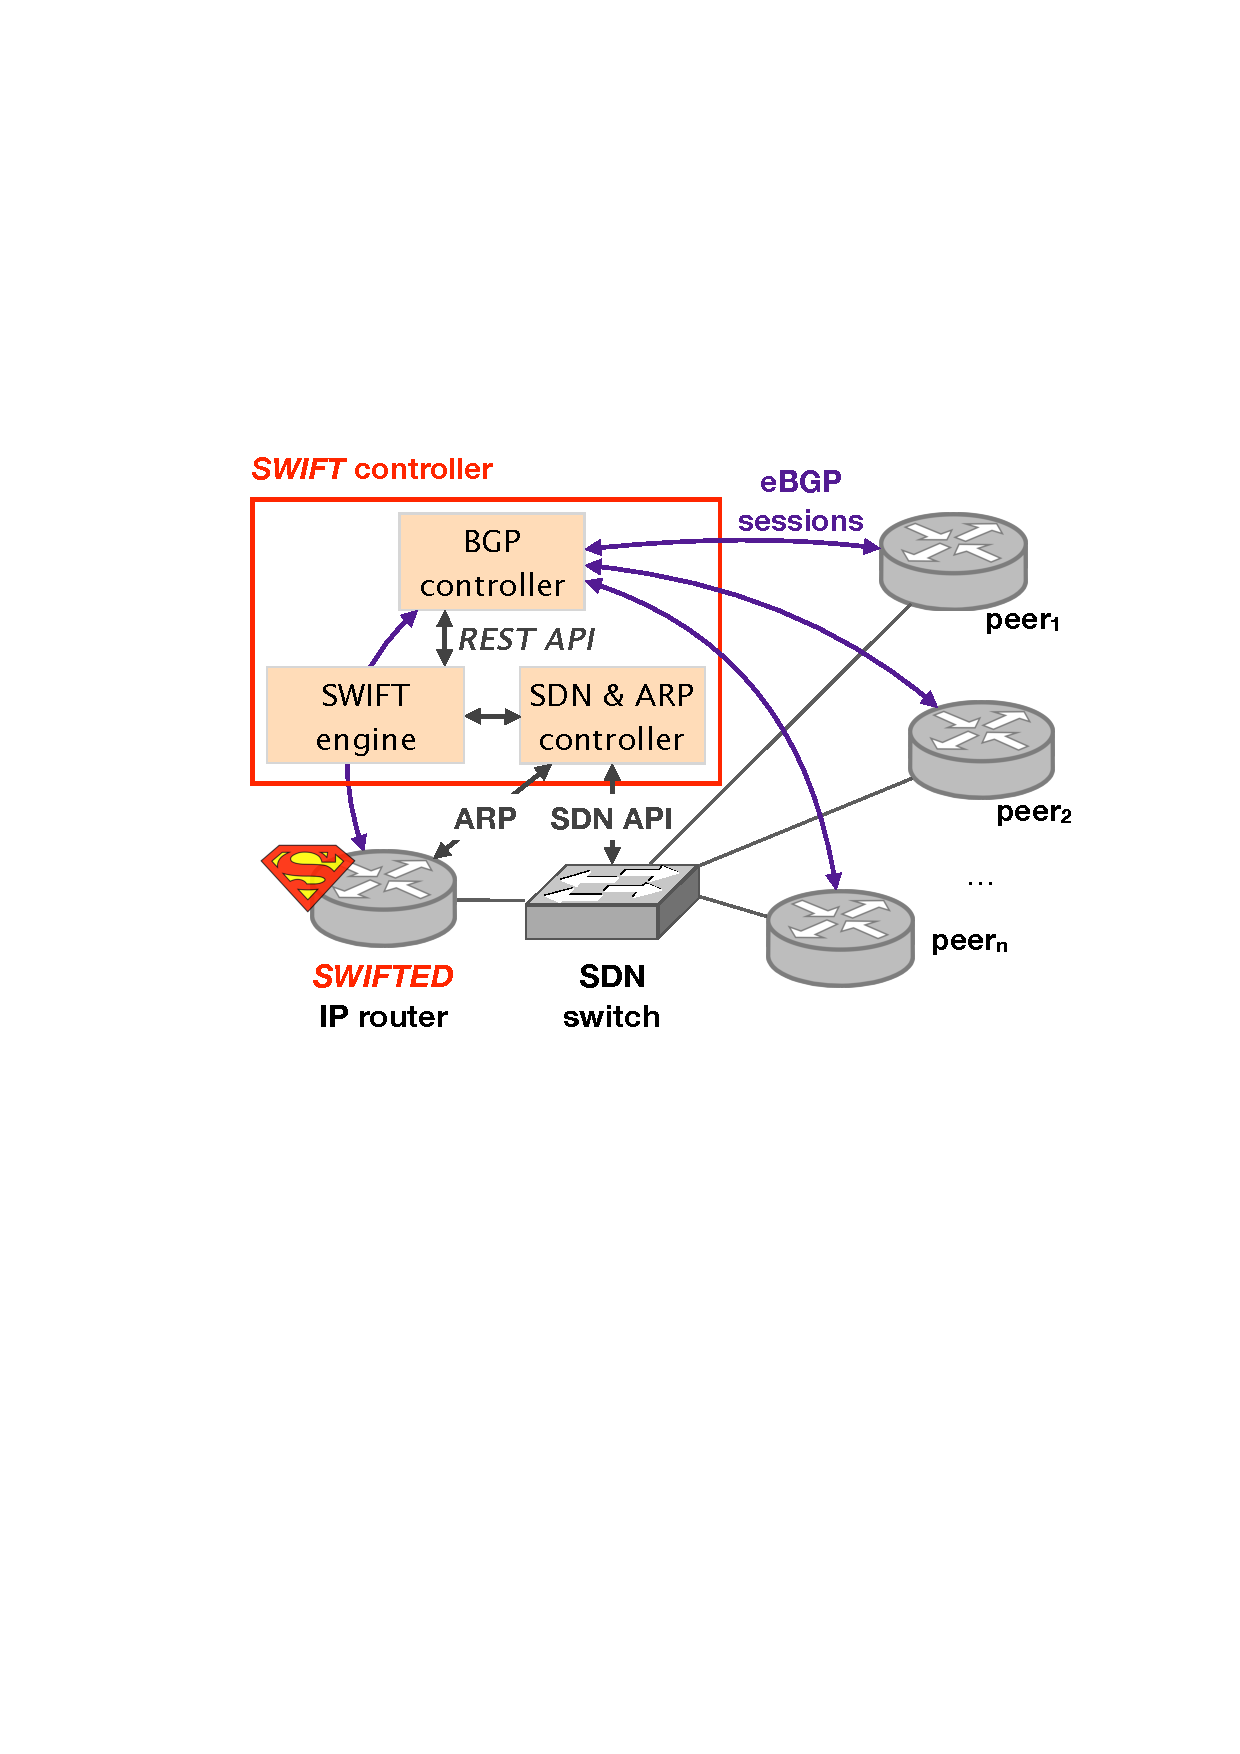
\includegraphics[scale = 0.5]{C:/Users/Philipp/SemesterProject/report/Figures/bckgrnd_swift_architecture.pdf}
\caption{Example topology of a swifted router}
\end{figure}

The Swift Controller has two main modules: the burst prediction algorithm and the encoding of routing information. 

\subsection{\label{chapter2:Swift:encoding of routing information}encoding of routing information}
Swift similarly to the iSDX uses virtual next-hops and the destination mac address to encode information about the packet's prefix.\\
For every prefix Swift encodes the AS-path up to a certain depth and the backup next-hops for each AS-link on that AS-path. This encoding is then mapped to a virtual next-hop. When the swifted router wants to send a packet to any prefix it will use the virtual next-hop assigned by Swift. The virtual next-hop directly maps to the destination mac address. 

\paragraph{\label{chapter2:Swift:Swift vmac}Swift vmac:}

\begin{tabular}{|r|l|}
  \hline 
  backup next-hops for AS-links & AS-path \\
  \hline
\end{tabular}


\begin{figure}[h]
\center
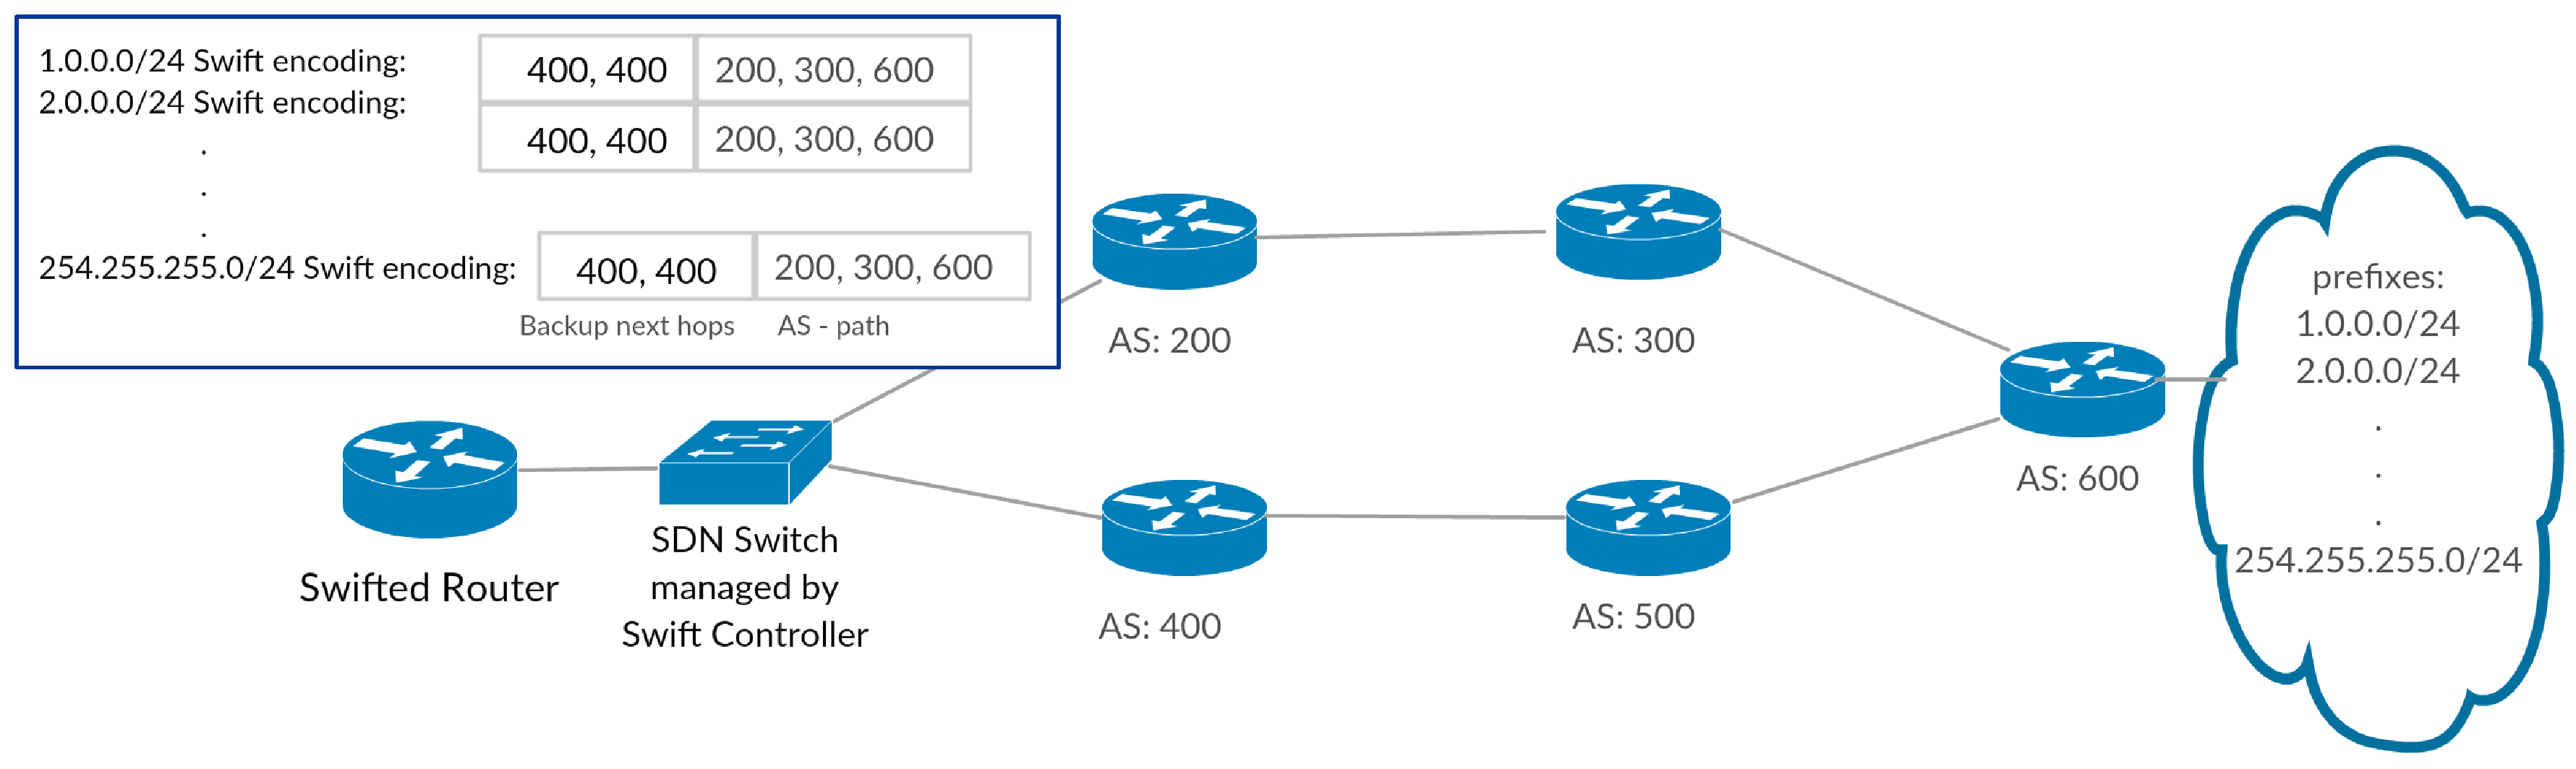
\includegraphics[scale = 0.24]{C:/Users/Philipp/SemesterProject/report/Figures/bckgrnd_swift_topology.pdf}
\caption{Example of the Swift vmac}
\end{figure}


\subsection{\label{chapter2:Swift:burst prediciton algorithm}burst prediction algorithm}
The burst prediction algorithm takes BGP updates. It uses the updates to build a AS-topology. Once enough withdrawals arrive in a time frame short enough to trigger a burst, the burst prediction algorithm uses the withdrawals and the AS-topology to predict the failed AS-link. \\
Upon predicting a failed link the Swift Controller pushes flow rules int the SDN switch matching on the failed AS-link and on the corresponding backup next-hop. \\
Every packet that traverses the failed link (has the failed AS-link in its AS-path encoding) will get rerouted to the backup neighbor.
\begin{figure}[h]
\center
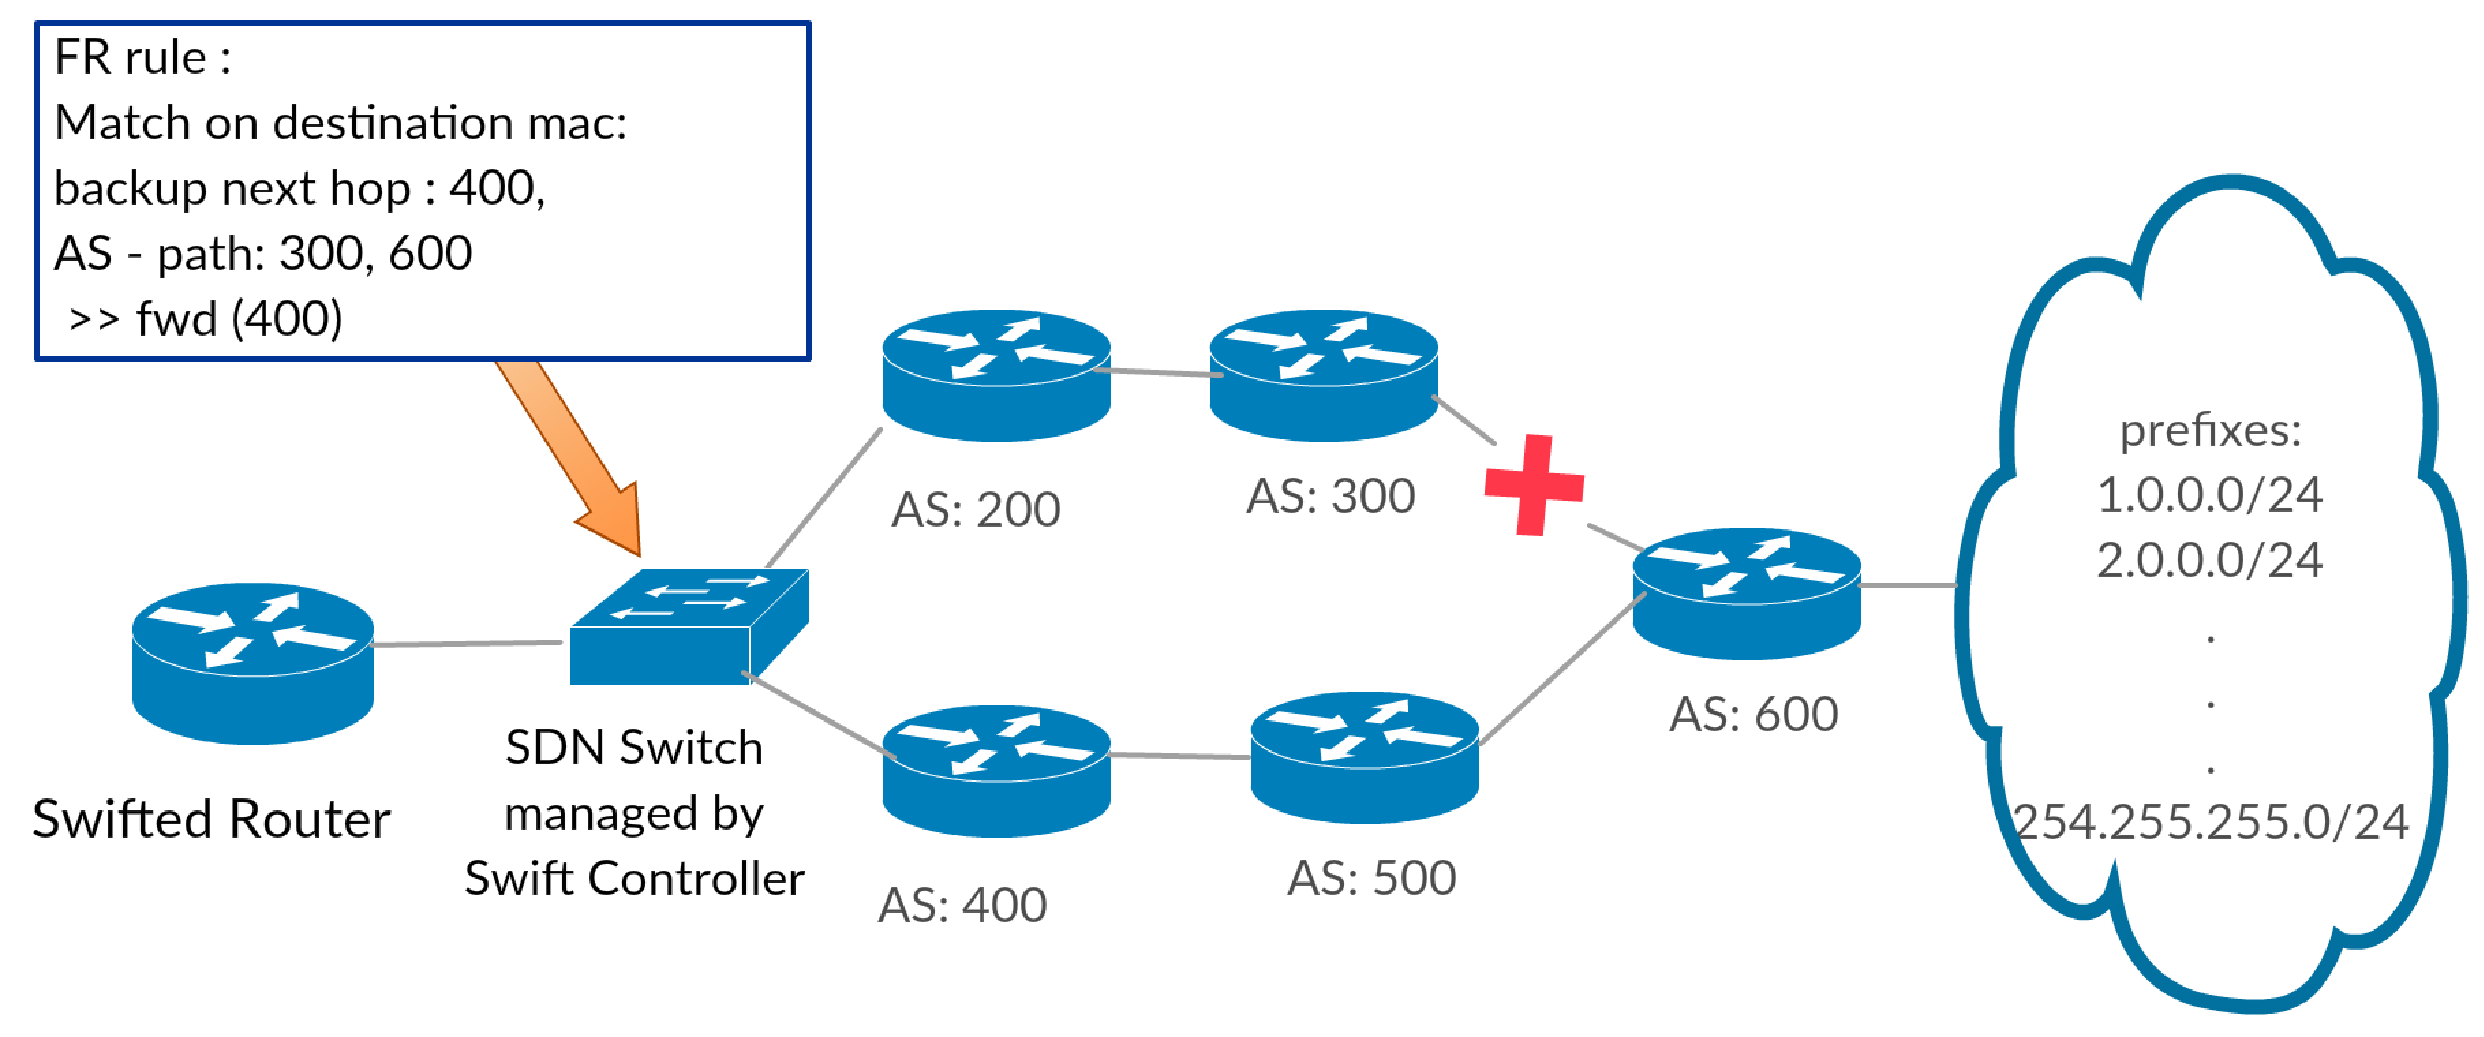
\includegraphics[scale = 0.36]{C:/Users/Philipp/SemesterProject/report/Figures/bckgrnd_swift_fr.pdf}
\caption{Example of a fast-reroute after BPA predicts the AS link 300 600 to be down}
\end{figure}

By predicting the failed and pushing fast-reroute rules instead of waiting for all withdraws to arrive, Swift reduces the convergence time of the swifted router significantly.


\section{\label{chapter2:Motivation}Motivation}

The iSDX takes a long time to converge upon remote failure. The main problem is that the iSDX needs to do some additional computing a traditional bgp router does not need to do. \\
When receiving a withdrawal the iSDX participant controller updates it's RIB, checks if the policy flow rules have changed and if the virtual next hop/vmac has changed. This additional computation adds a significant overhead to the convergence time of the iSDX. \\
Implementing Swift into the iSDX promises to significantly reduce the convergence time. Convergence time being the time until packets get sent to the correct participant and not into a black hole. \\
The main reason why implementing Swift in the iSDX is reasonable is their similar architecture. Both the iSDX and Swift use a SDN switch to program flow rules to steer traffic. They both are connected to BGP speaking routers and receive BGP updates from them. Swift and iSDX both use the destination mac address to encode information about a prefix and use the next-hop to map this vmac to a prefix. In addition the swift framework allows multiple swifted routers to be connected to the SDN switch, which in the iSDX's case means that all the participants will benefit swift.





